\chapter{Nested clade analysis}

In a very influential paper Avise et al.~\cite{Avise-etal-1987}
introduced the term ``phylogeography'' to refer to evolutionary
studies lying at the interface of population genetics and phylogentic
systematics. An important property of molecular sequences is that the
degree of difference among them contains information about their
relatedness. Avise et al.\ proposed combining information derived from
the phylogenetic relationship of molecular sequences with information
about where the sequences were collected from to infer something about
the biogeography of relationships among populations within
species. Figure~\ref{fig:bowfin} provides an early and straightforward
example.\index{phylogeography}

\begin{figure}
\begin{center}
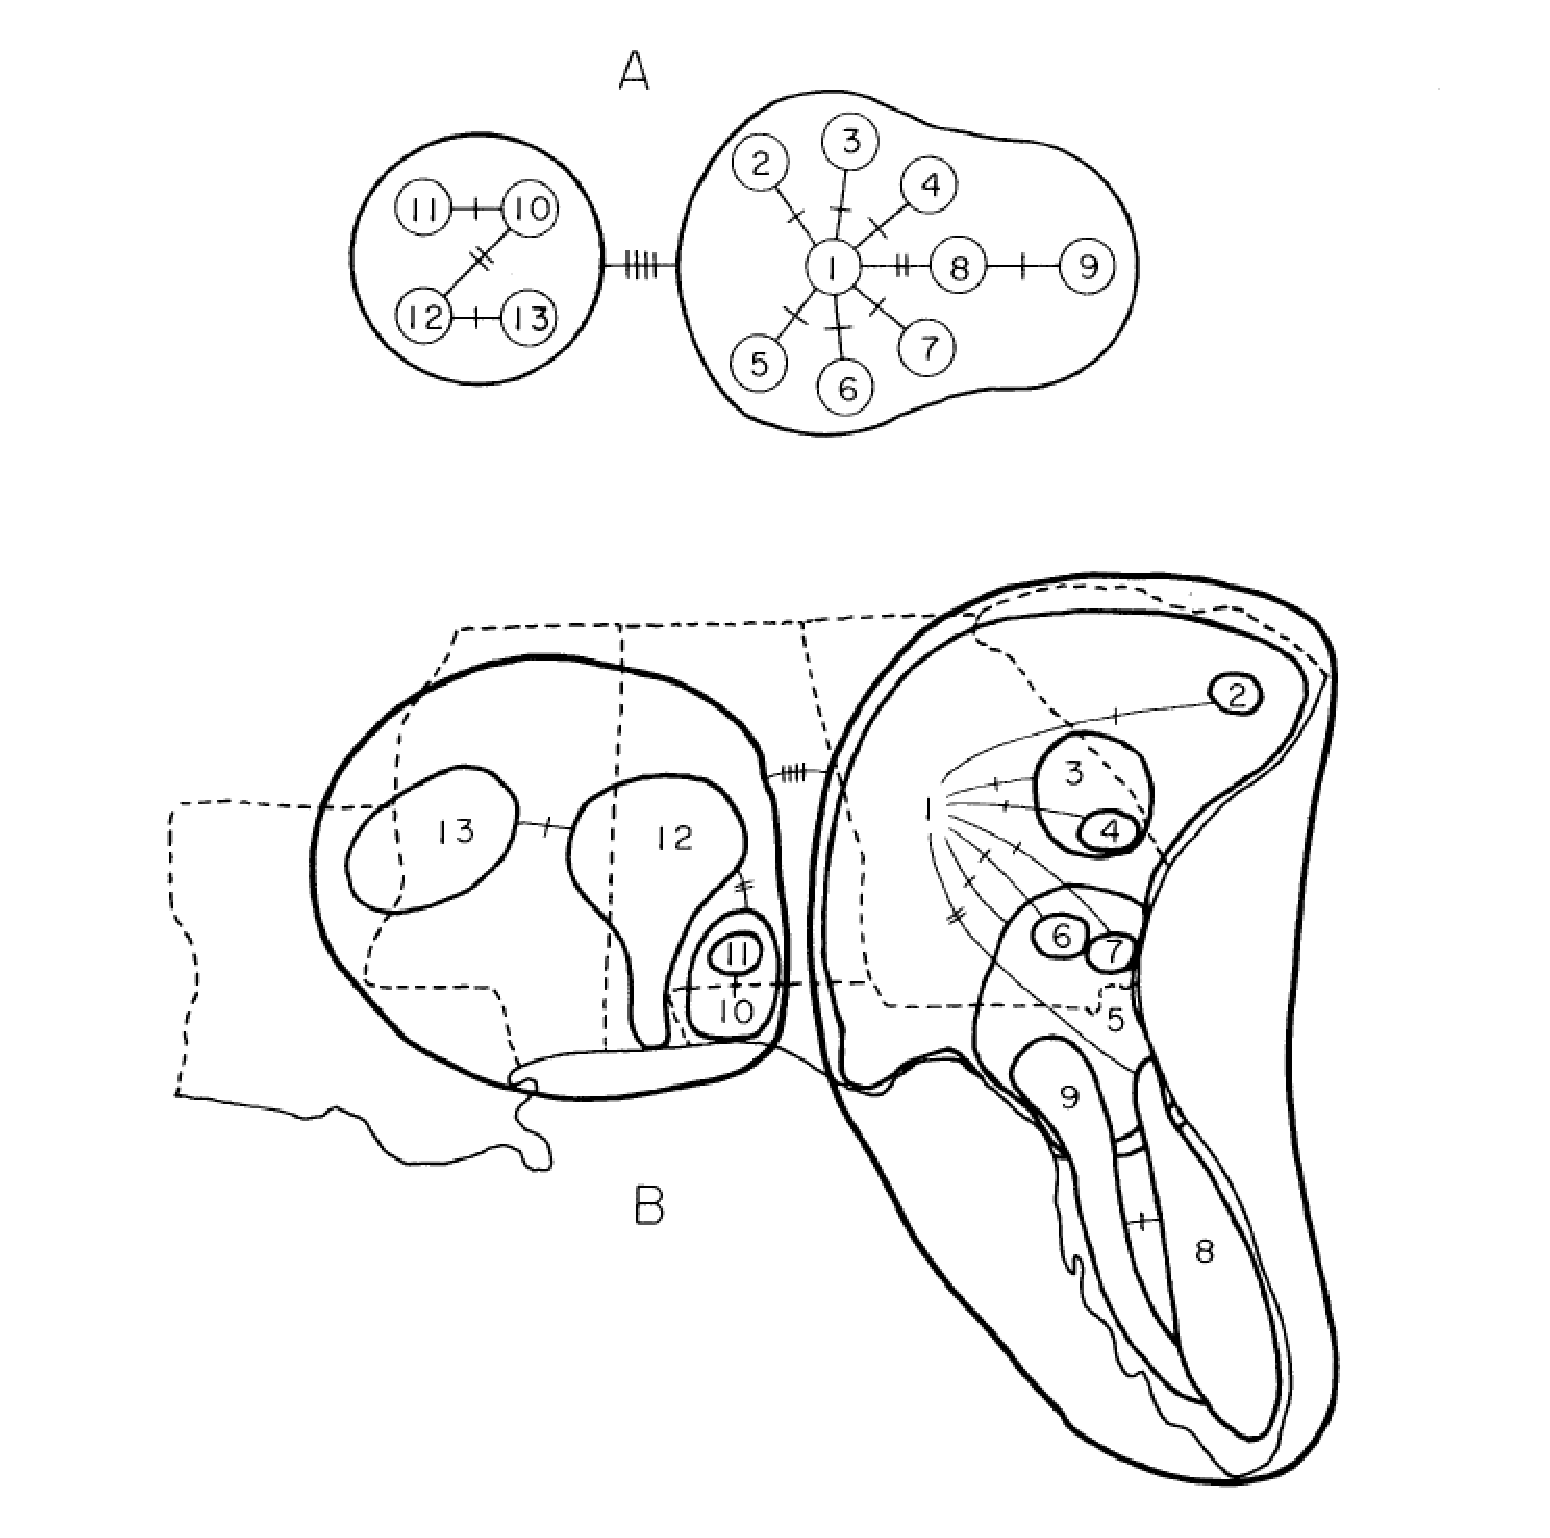
\includegraphics[width=0.425\textwidth]{bowfin-phylogeography.eps}
\end{center}
\caption{A phylogeographic analysis of 75 bowfins, {\it Amia calva\/},
  sampled from the southeastern United States. {\bf A.} A parsimony
  network connecting the 13 mtDNA haplotypes identified from the
  sample. {\bf B.} The geographical distribution of the
  haplotypes.}\label{fig:bowfin}\index{Amia@\textit{Amia}!\textit{calva}}
\end{figure}

The data are from bowfins, {\it Amia calva}, and consist of mtDNA
haplotypes detected by restriction site mapping. There are two highly
divergent groups of haplotypes separated from one another by a minimum
of four restriction site differences. Moreover, the two sets of
haplotypes are found in areas that are geographically
disjunct. Haplotypes 1-9 are found exclusively in the eastern portion
of the range, while haplotypes 10-13 are found exclusively in the
western part of the range. This pattern suggests that the populations
of bowfin in the two geographical regions have had independent
evolutionary histories for a relatively long period of
time. Interestingly, this disjunction between populations west and
east of the Appalachicola River is shared by a number of other
species, as are disjunctions between the Atlantic and Gulf coasts, the
west and east sides of the Tombigbee River, the west and east sides of
the Appalachian mountains, and the west and east sides of the
Mississippi River~\cite{Soltis-etal-2006}.

Early analyses often provided very clear patterns, like the one in
bowfins. As data accumulated, however, it became clear that in some
species it was necessary to account for differences in frequency, not
just presence {\it versus\/} absence of particular haplotypes. We saw
this in the application of AMOVA to mtDNA haplotype variation in
humans. These approaches have two critical things in common:

\begin{itemize}

\item Haplotype networks are constructed as minimum-spanning
  (parsimony) networks without consideration as to whether assuming a
  parsimonious reconstruction of among haplotype differences is
  reasonable.\footnote{For those of you who are familiar with
    molecular phylogenetics as it is usually applied, there's another
    important difference. Not only are these parsimony networks. They
    are networks in which some haplotypes are regarded as ancestral to
    others, i.e., haplotypes appear not only at the tips of a tree,
    but also at the nodes.}

\item The relationship between geographical distributions and
  haplotypes contains information about the history of those
  distributions, but there is no formal way to assess different
  interpretations of that history.

\end{itemize}

Nested-clade analysis (NCA) has become a widely used technique for
phylogeographic analysis because it provides methods intended to
assess each of those concerns~\cite{Templeton-2004}.\footnote{It
  continues to produce networks in which some haplotypes are ancestral
  to others, but in this context, such an approach is reasonable. Ask
  me about it if you're interested in why it's reasonable.} In broad
outline the ideas are pretty simple:\index{nested clade analysis}

\begin{itemize}

\item Use statistical parsimony to construct a statistically
  supportable haplotype network.

\item Identify nested clades, test for an association between
  geography and haplotype distribution, and work through an inference
  key to identify the processes that could have produced the
  association.

\end{itemize}

As we'll see, implementing these simple ideas poses some
challenges.\footnote{When we talk about statistical phylogeography,
  you'll see an alternative approach to addressing the concerns NCA
  was intended to address.}

\section*{Statistical parsimony}

Templeton et al.~\cite{Templeton-etal-1992} lay out the theory and
procedures involved in statstical parsimony in great detail. As with
NCA in general, the details get a little complicated. We'll get to
those complications soon enough, but again as with NCA in general the
basic ideas are pretty simple:\index{statistical parsimony}\index{nested clade analysis!statistical parsimony}\index{TCS parsimony}

\begin{itemize}

\item Evaluate the limits of parsimony, i.e., the number of mutational
  steps that can be reliably inferred without having to worry about
  multiple substitutions.

\item Construct ``the set of parsimonious and non-parsimonious
  cladograms that is consistent with these limits''~(p.\
  619).\footnote{Makes you wonder a little about why it's called
  statistical parsimony if some of the reconstructed cladograms aren't
  parsimonious, doesn't it?}

\end{itemize}

So why use parsimony? Within species the time for substitutions to
occur is relatively short. As a result, it may be reasonable to assume
that we don't have to worry about multiple substitutions having
occurred, at least between those haplotypes that are the most closely
related. To ``identify the limits of parsimony'' we first estimate
$\theta=4N_e\mu$ from our data. Then we plug it into a formula that
allows us to assess the probability that the difference between two
randomly drawn haplotypes in our sample is the result of more than one
substituion.\footnote{If you're interested, you can find the formula
  for restriction site differences in equation (1), p. 620.} If that
probability is small, say less than 5\%, we can connect all of the
haplotypes into a parsimonious network, i.e., one that involves only
single substitutions between haplotypes~(some of which may be
hypothetical and unobserved).

More likely than not, we won't be able to connect all of the
haplotypes parsimoniously, but there's still a decent chance that
we'll be able to identify subsets of the haplotypes for which the
assumption of parsimonious change is reasonable. Templeton et
al.~\cite{Templeton-etal-1992} suggest the following procedure to
construct a haplotype network:\index{statistical parsimony!haplotype network}\index{TCS parsimony}

\begin{description}

\item[Step 1:] Estimate $P_1$ the probability that haplotype pairs
  differing by a single change are the result of a single
  substitution. If $P_1 > 0.95$, as is likely, connect all pairs of
  haplotypes that differ by a single change. There may be ambiguities
  in the reconstruction, including loops. Keep these in the
  network~(Figure~\ref{fig:haplotype-network}).

\begin{figure}
\begin{center}
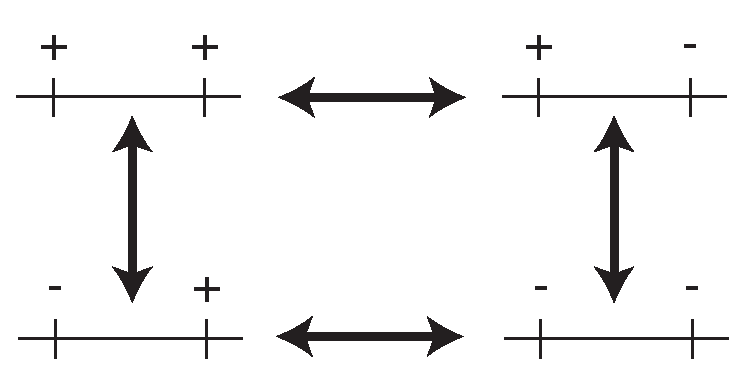
\includegraphics[width=0.425\textwidth]{haplotype-network.eps}
\end{center}
\caption{An example of four haplotypes connected in a single-step
  network showing that two paths are possible between haplotypes that
  differ in two positions.}\label{fig:haplotype-network}
\end{figure}


\item[Step 2:] Identify the products of recombination by inspecting
  the 1-step network to determine if postulating recombination between
  a pair of sequences can remove ambiguity identified in step 1.

\item[Step 3:] Augment $j$ by one and estimate $P_j$. If $P_j > 0.95$,
  join $j-1$-step networks into a $j$-step network by connecting
  the two haplotypes that differ by $j$ steps. Repeat until either all
  haplotypes are included in a single network or you are left with two
  or more non-overlapping networks.

\item[Step 4:] If you have two or more networks left to connect,
  estimate the smallest number of non-parsimonious changes that will
  occur with greater than 95\% probability, and connect the networks.

\end{description}

\noindent Refer to Templeton et al.~\cite{Templeton-etal-1992} for
details of the calculations. Figure~\ref{fig:amy-tcs} provides an
example of the kind of network that may result from this
analysis.\index{Drosophila@\textit{Drosophila}!\textit{melanogaster}}\index{statistical parsimony!example}

\begin{figure}
\begin{center}
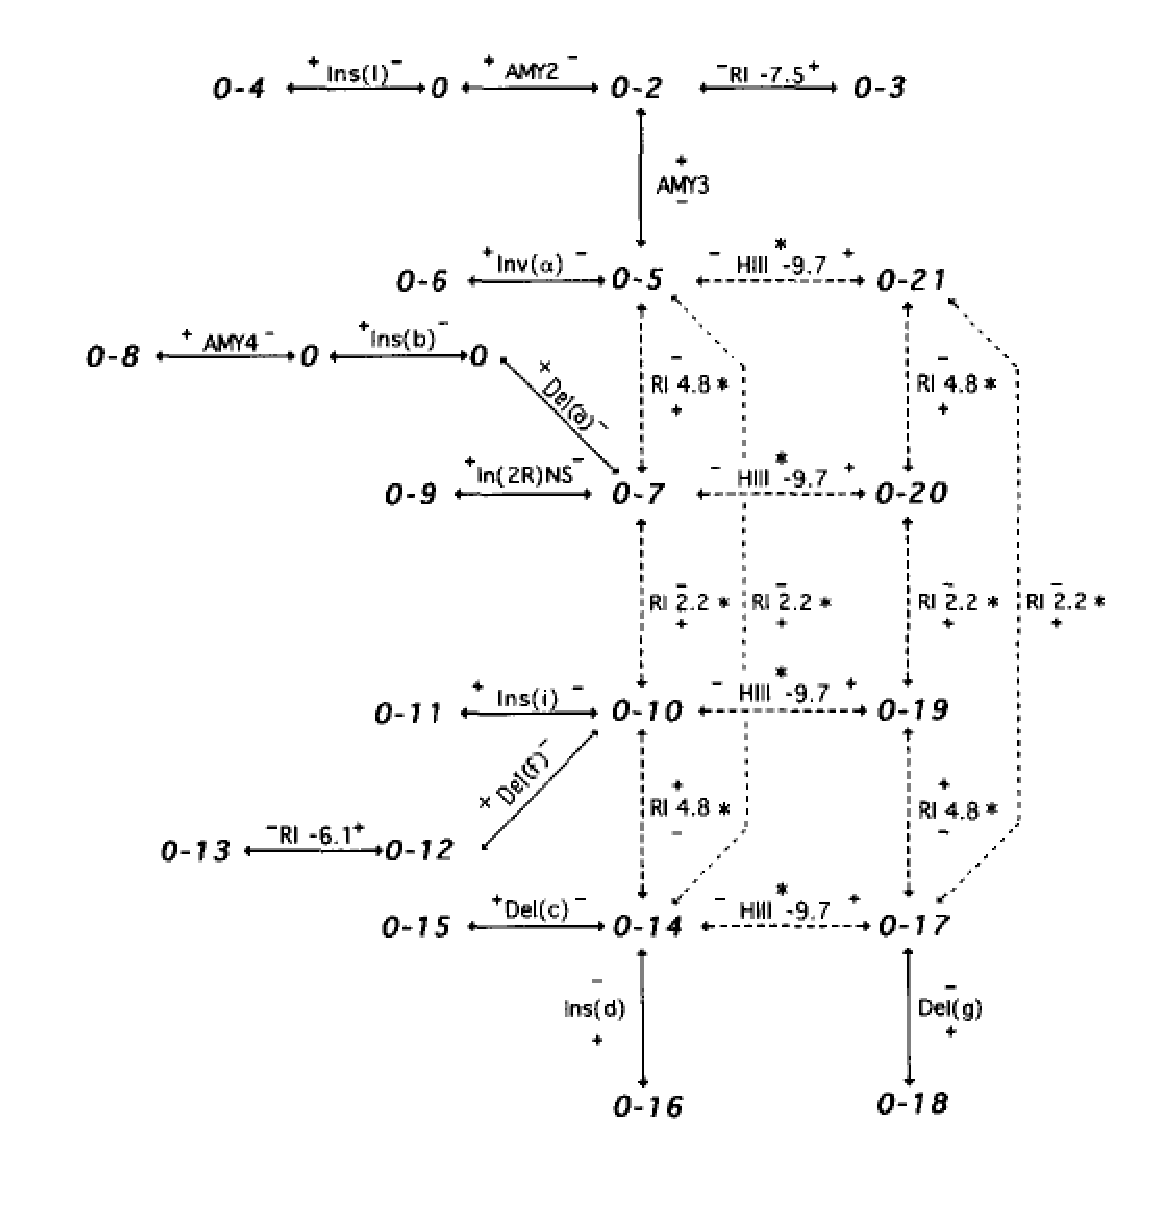
\includegraphics[height=12cm]{amy-tcs.eps}
\end{center}
\caption{Statistical parsimony network for the {\it Amy\/} locus of
  {\it Drosophila melanogaster}.}\label{fig:amy-tcs}
\end{figure}

\section*{Nested clade analysis}

Once we have constructed the haplotype network, we're then faced with
the problem of identifying nested clades. Templeton et
al.~\cite{Templeton-etal-1987} propose the following algorithm to
construct a unique set of nested clades:\index{nested clade analysis!constructing nested clades}

\begin{description}

\item[Step 1.] Each haplotype in the sample comprises a 0-step clade,
  i.e., each copy of a particular haplotype in the sample is separated
  by zero evolutionary steps from other copies of the same
  haplotype. ``Tip'' haplotypes are those that are connected to only
  one other haplotype. ``Interior'' haplotypes are those that are
  connected to two or more haplotypes. Set $j=0$

\item[Step 2.] Pick a tip haplotype that is not part of any $j+1$-step
  network.

\item[Step 3.] Identify the interior haplotype with which it is
  connected by $j+1$ mutational steps.

\item[Step 4.] Identify all tip haplotypes connected to that interior
  haplotype by $j+1$ mutational steps.

\item[Step 5.] The set of all such tip and interior haplotypes
  constitutes a $j+1$-step clade.

\item[Step 6.] If there are tip haplotypes remaining that are not part
  of a $j+1$-step clade, return to step 2.

\item[Step 7.] Identify internal $j$-step clades that are not part of
  a $j+1$ step clade and are separated by $j+1$ steps.

\item[Step 8.] Designate these clades as ``terminal'' and return to
  step 2.

\item[Step 9.] Increment $j$ by one and return to step 2.

\end{description}

\noindent That sounds fairly complicated, but if you look at the
example in Figure~\ref{fig:nca-nesting}, you'll see that it isn't all
{\it that\/} horrible.

\begin{figure}
\begin{center}
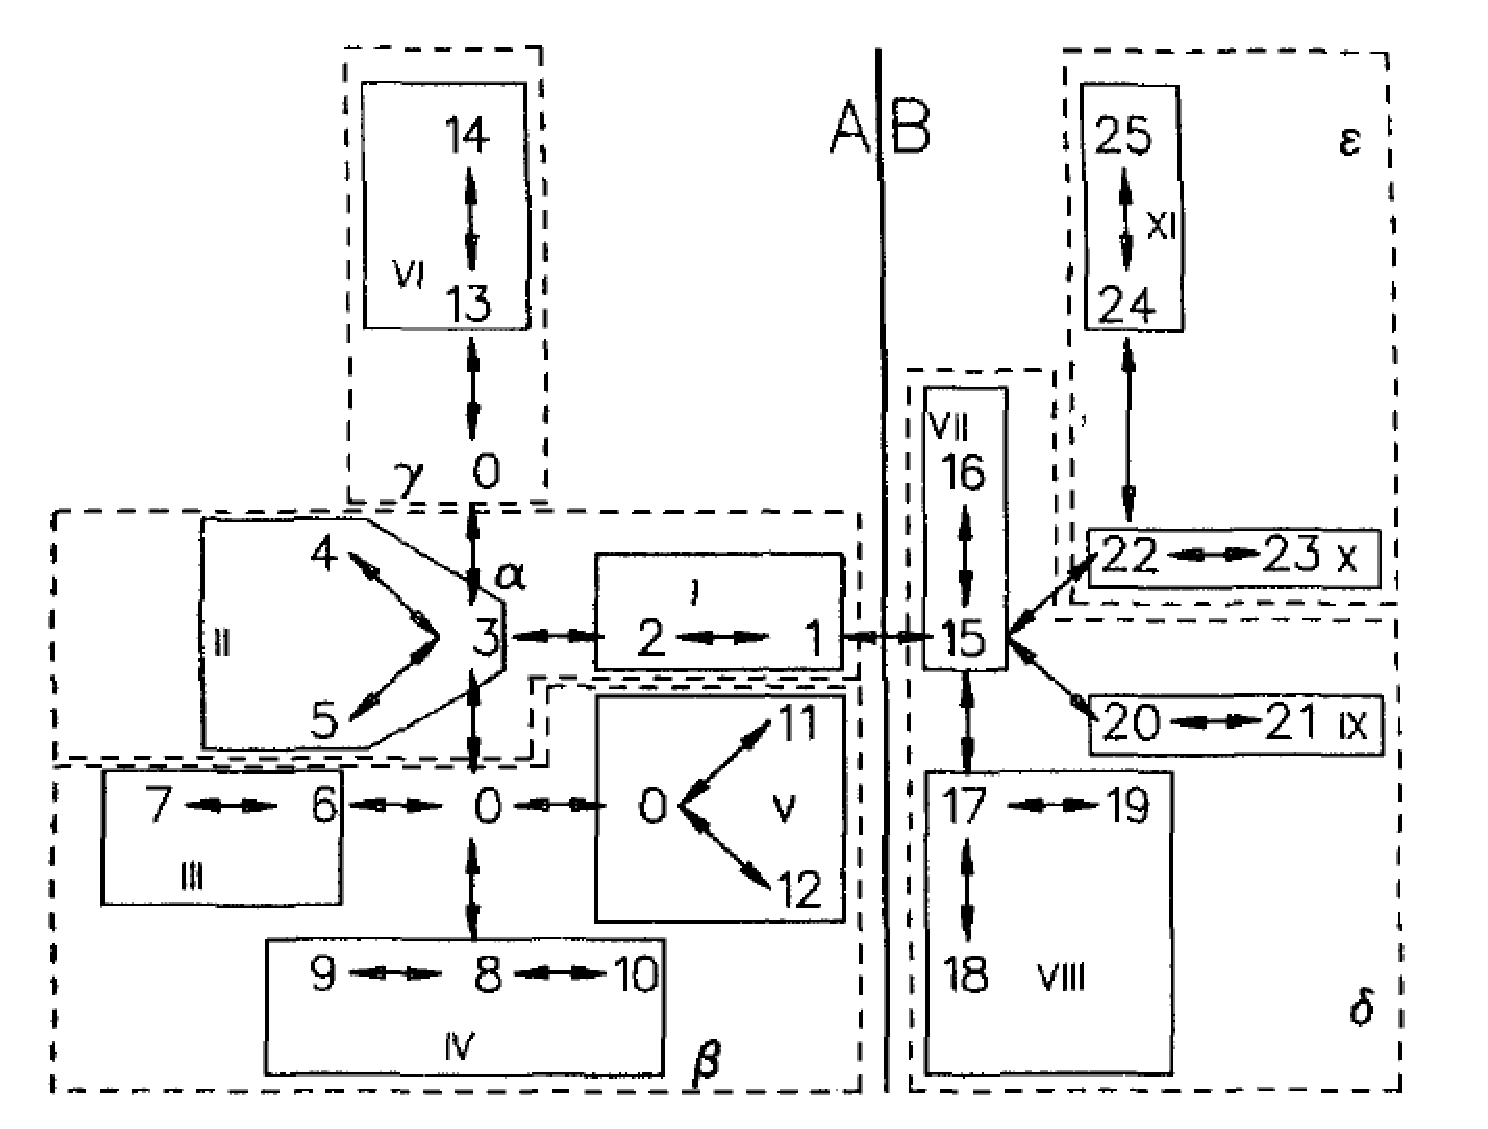
\includegraphics[height=8cm]{nca-nesting.eps}
\end{center}
\caption{Nesting of haplotypes at the {\it Adh\/} locus in {\it
    Drosophila melanogaster}.}\label{fig:nca-nesting}
\end{figure}

This algorithm produces a set of nested clades, i.e., a 1-step clade
is contained within a 2-step clade, a 2-step clade is contained within
a 3-step clade, and so on. Once such sets of nested clades have been
identified, we can calculate statistics related to the geographical
distribution of each clade in the sample. Templeton et
al.~\cite{Templeton-etal-1995} define two statistics that are used in
an inferential key~(the most recent version of the key is
in~\cite{Templeton-2004}; see Figure~\ref{fig:nca-calc}):

\begin{description}

\item[Clade distance] The average distance of each haplotype in the
  particular clade from the center of its geographical
  distribution. ``Distance'' may be the great circle distance or it
  might be the distance measured along a presumed dispersal
  corridor. The clade distance for clade $X$ is symbolized $D_c(X)$,
  and it measures how far this clade has spread.\index{clade
    distance}\index{nested clade analysis!clade distance}

\item[Nested clade distance] The average distance of the center of
  distribution for this haplotype from the center of distribution for
  the haplotype within which it is nested. So if clade $X$ is nested
  within clade $Y$, we calculate $D_n(X)$ by determinining the
  geographic center of clades $X$ and clade $Y$ and measuring the
  distance between those centers. $D_n(X)$ measures how far the clade
  has changed position relative to the clade from which it
  originated.\index{nested clade analysis!nested clade distance}

\end{description}

\begin{figure}
\begin{center}
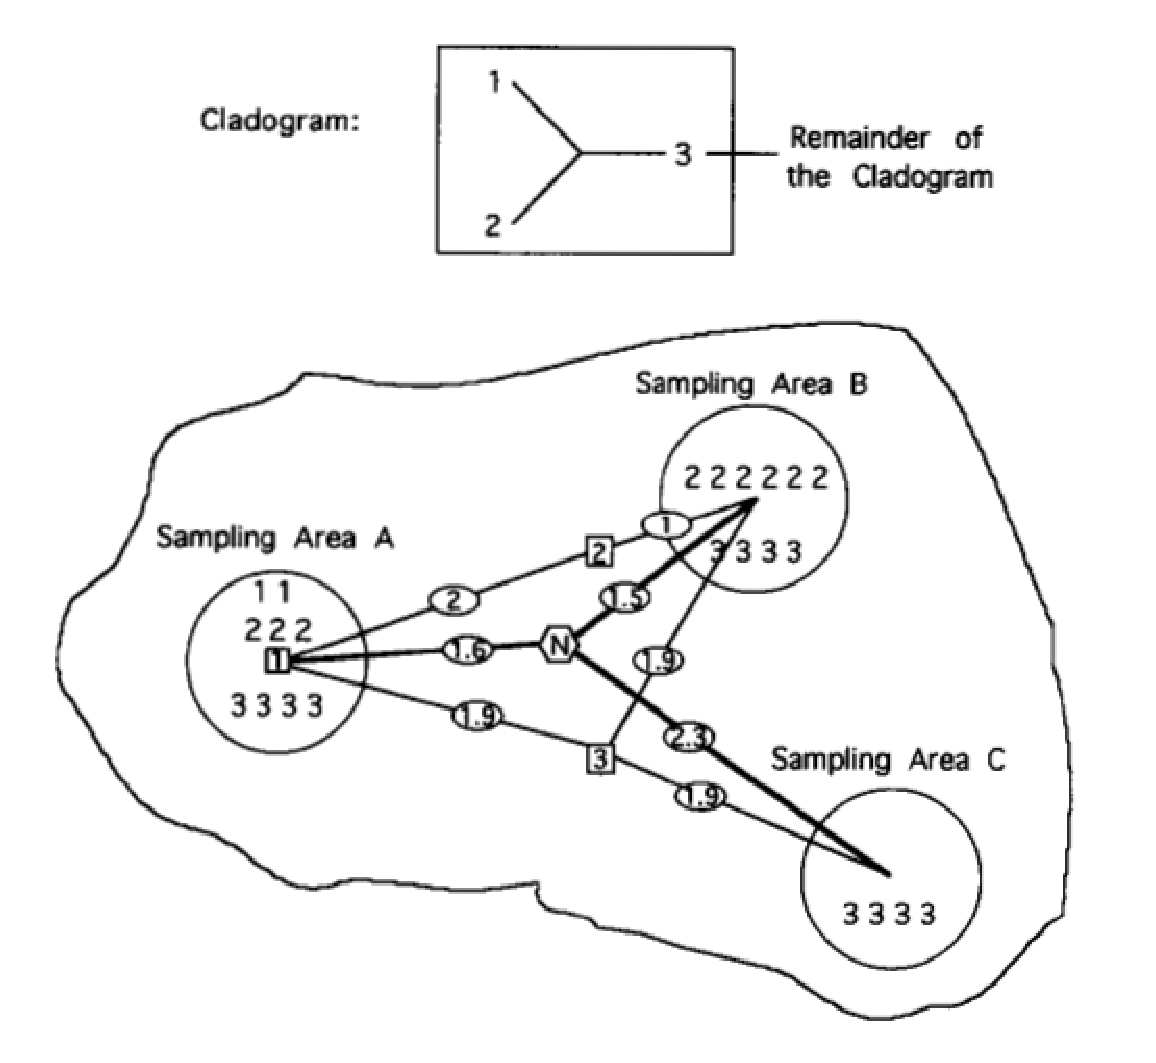
\includegraphics[scale=0.4]{nca-calculations.eps}
\end{center}
\caption{Each number corresponds to a haplotype in the
  sample. Haplotypes 1 and 2 are ``tip'' haplotypes. Haplotype 3 is an
  interior haplotype. The numbers in square boxes illustrate the
  center for each 0-step clade (a haplotype). The hexagonal ``N''
  represents the center for the clade containing 1, 2, and 3. Numbers
  in ovals are the distances from the center of each collecting area
  to the clade center. $D_c(1)=0$, $D_c(2)=(3/9)(2)+(6/9)(1)=1.33$,
  $D_c(3) = (4/12)(1.9) + (4/12)(1.9) + (4/12)(1.9)=1.9$. $D_n(1) =
  1.6$, $D_n(2)=(3/9)(1.6)+(6/9)(1.5)=1.53$, $D_n(3)=
  (4/12)(1.6)+(4/12)(1.5)+(4/12)(2.3)=1.8$.}\label{fig:nca-calc}
\end{figure}


Once you've calculated these distances, you randomly permute the
clades across sample locations. This shuffles the data randomly,
keeping the number of haplotypes and the sample size per location the
same as in the orignal data set. For each of these permutations, you
calculate $D_c(X)$ and $D_n(X)$. If the observed clade distance, the
observed nested clade difference, or both are significantly different
from expected by chance, then you have evidence of (a) geographical
expansion of the clade (if $D_c(X)$ is greater than null expectation)
or (b) a range-shift (if $D_n(X)$ is greater than null
expectation). Using these kinds of statistics, you run your data set
through Templeton's inference key to reach a conclusion. For example,
applying this procedure to data from {\it Ambystoma tigrinum}~(Figure
\ref{fig:ambystoma}), Templeton et al.~\cite{Templeton-etal-1995}
construct the scenario in Figure~\ref{fig:ambystoma-inference}.

\begin{figure}
\begin{center}
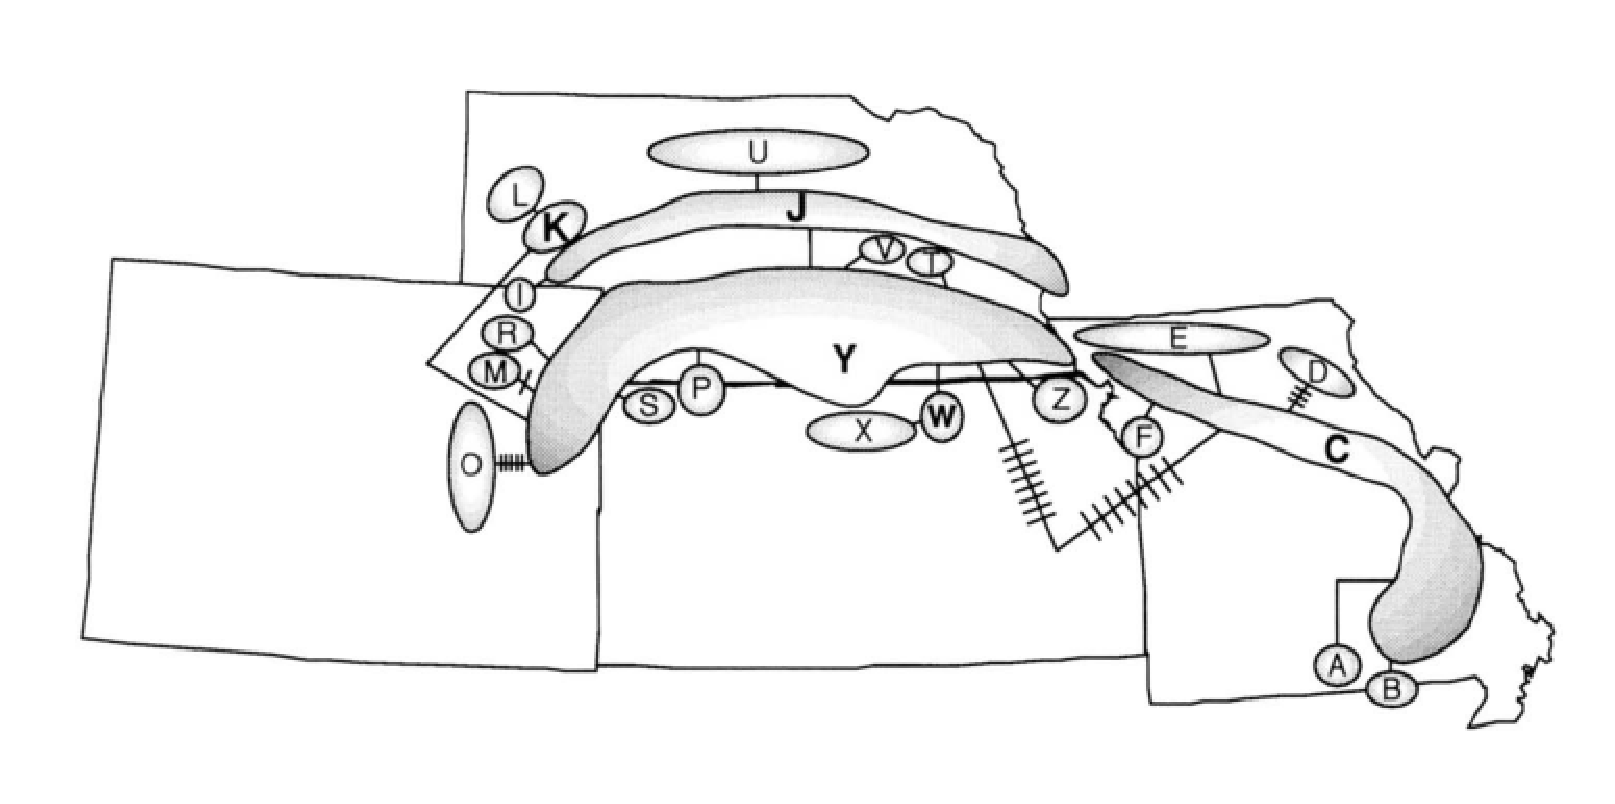
\includegraphics[height=6cm]{ambystoma.eps}
\end{center}
\caption{Geographic distribution of mtDNA haplotypes in {\it Ambystoma
    tigrinum}.}\label{fig:ambystoma}\index{Ambystoma@\textit{Ambystoma}!\textit{tigrinum}}
\end{figure}

\begin{figure}
\begin{center}
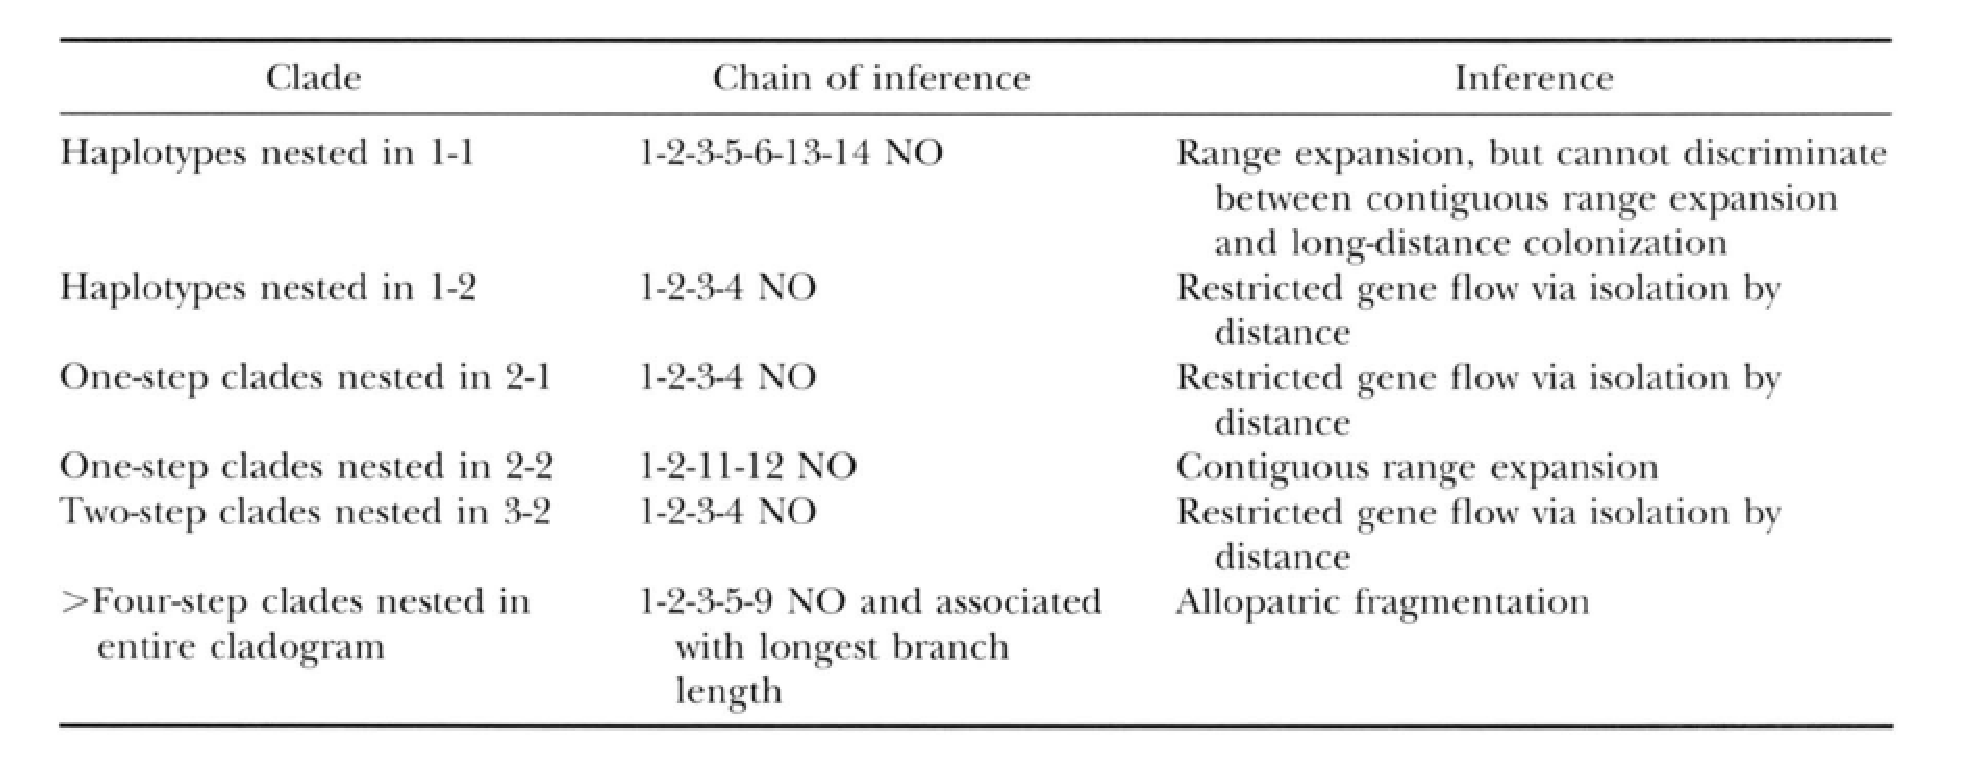
\includegraphics[height=6cm]{ambystoma-inference.eps}
\end{center}
\caption{Inference key for {\it Ambystoma
    tigrinum}.}\label{fig:ambystoma-inference}\index{Ambystoma@\textit{Ambystoma}!\textit{tigrinum}}
\end{figure}

